\chapter[Implementazioni OpenMp: Prodotto Simbolico]
{Implementazioni OpenMp:\\Prodotto Simbolico}
\label{ChSymbProduct}\label{chSpMMSymb}
In questa sezione si descrivono alcune implementazioni che ho realizzato per 
il calcolo del \nnnz del prodotto tra matrici sparse, introdotto precedentemente in \refbf{ChExistingTecqs:symbMul}.\\
In letteratura è consueto utilizzare la terminologia di prodotto simbolico 
per indicare il calcolo esatto della dimensione della matrice risultante all'operazione di SpMM.\\
%naming agree
Nel seguito si indicherà con prodotto simbolico, la generale operazione di determinare, 
con un bound o con precisione, la dimensione del Prodotto tra matrici sparse.\\
%TODO ANCHE IN MAIN O INTRODUZIONE O BREVE DESCRIZIONE DI OGNI CAPITOLO?
Come verrà descritto nel dettaglio in \refbf{chSpMMAux:multiImpl}, 
al fine di avere la massima efficienza nella generazioni
di multiple implementazioni dello stesso codice a compile-time, 
per supportare l'integrazione di tutte le implementazioni descritte in un progetto fortran come AMG4PSBLAS  \amgforpsblas,
saranno presenti nei frammenti di codice successivi macro come \verb|CAT OFF_F|,
necessarie ad ottenere molteplici versione del codice a tempo di pre processamento.\\
%-- Intro END ---------------------------------------------------------------------------
\voidLine
\label{chSpMMSymb:outputDetailLevel} %output diversi del prodotto simbolico in base al tipo di fase num.
In base al tipo di implementazione del prodotto numerico e di partizionamento dei dati tra i thread,
è necessaria una fase simbolica di SpMM per calcolare il \nnnz a livello di:\\
\begin{enumerate}
	\item	
		intere matrici $C$ e $\hat{C}$
	\item 	righe di $C$ e $\hat{C}$
	\item 	partizioni di colonne in righe di $C$ e $\hat{C}$
\end{enumerate}
Il livello di output prodotto da ogni livello può essere inclusivo di quello prodotto dal livello inferiore.\\
La necessità di avere una predizione della dimensione del risultato con un dettaglio differente 
è dovuta al tipo di implementazione usata per il Prodotto Numerico e 
sarà descritta successivamente in \refbf{chSpMMNum:funcsMultiImplePurpose}.\\
La numerazione appena introdotta per il livello di dettaglio dell'output del prodotto simbolico 
sarà riferita nel seguito.\\

\section{UpperBound} \label{chSpMMSymb:UpperBound}
Come descritto in \refbf{ChExistingTecqs:symbUpperBound}, la determinazione di un limite superiore al \nnnz 
del risultato di SpMM è computabile rapidamente e semplicemente.
\voidLine
Nel caso di dover determinare un prodotto simbolico a livello 1 o 2 %(secondo la numerazione appena introddota\refbf{chSpMMSymb:outputDetailLevel} )
si ha un costo computazionale proporzionale al \nnnz di $A$.\\
\voidLine
Nel caso di dover calcolare un bound per ogni partizione di colonne di ogni riga di $C$ e $\hat{C}$,
per implementazioni della fase numerica con partizionamento bidimensionale delle matrici, ho utilizzato
il seguente approccio.\\
Un bound superiore della dimensione della k-esima partizione di colonne di $c_{i*}$ 
è calcolabile restringendo la formula $ | I_i(C) |~\leq~\sum\limits_{ j \in I_i(A) }  | I_j(B) | $
all' sottoinsieme di elementi \nnz relativi della k-esima partizione di colonne di B.\\
Segue l'implementazione di questa operazione.\\
\begin{lstlisting}
/* 
 * return matrix @A.M x @gridCols of upper bounded num of non zeros
 * for each of the @gridCols col partitions of the output matrix AB = @A * @B rows
 * also appended at the end for the cumulative total size of the matrix AB 
 */
inline idx_t* CAT(spMMSizeUpperboundColParts_,OFF_F)
  (spmat* A,spmat* B,ushort gridCols,idx_t* bColPartOffsets){
    idx_t* rowPartsSizes = calloc((A->M*gridCols +1),  sizeof(*rowPartsSizes));
    if (!rowPartsSizes){
        ERRPRINT("rowPartsSizes calloc errd\n");
        return NULL;
    }

    idx_t fullMatBound = 0;
    #pragma omp parallel for schedule(static) reduction(+:fullMatBound)
    for (idx_t r=0;  r<A->M; r++){
        //for each A.row -> sum B.colParts lens     
        for (idx_t jj=A->IRP[r]-OFF_F,j,rlen;  jj<A->IRP[r+1]-OFF_F; jj++){
            j = A->JA[jj] - OFF_F;
            for (idx_t gc=0,bPartID=IDX2D(j,gc,gridCols);  gc < gridCols; gc++,bPartID++){
                rlen = bColPartOffsets[bPartID+1] - bColPartOffsets[bPartID];
                rowPartsSizes[ IDX2D(r,gc,gridCols) ]   += rlen;
                fullMatBound    += rlen;
            }
        }
    }
    rowPartsSizes[ A->M*gridCols ]  = fullMatBound;
    return rowPartsSizes;
}
\end{lstlisting}
Nella funzione precedente viene sfruttato un partizionamento 2D di B mediante una matrice di offset, \vvv{bColPartOffsets},
dove l'elemento $i,j$ è l'indice dell'elemento \nnz iniziale della 
j-esima partizione di colonne della i-esima riga.
Questa struttura di supporto è descritta nel dettaglio insieme ad altre metodologie di partizionamento 
per matrici sparse in \refbf{chSpMMAux:CSR2DPARTI}.\\
Il bound sulla \vvv{gc}-esima partizione della \vvv{r}-esima riga di $C$ 
è calcolato a riga 21, come precedentemente descritto.\\ 
\label{chSpMMSymb:OMPSetupCosts}
Per ogni livello di dettaglio del calcolo del prodotto simbolico, viene calcolata anche la dimensione
totale della matrice $C$, mediante la riduzione offerta da OpenMp con la clausola \vvv{reduction(+:..)}.\\
In generale l'overhead relativo ai vari componenti di OpenMp da istanziare per effettuare solamente
una operazione di riduzione possono precludere un beneficio prestazionale per input piccoli.
\\Tuttavia, l'uso di questa clausola all'interno di un ciclo parallelizzato più ampio può ammortizzare
l'overhead di inizializzazione di OpenMp, dando un beneficio di performance.\\
%Per comodità come ultimo elemento dell'array di output dell'operazione, 


\section{Calcolo Accurato}
Per il prodotto simbolico accurato, focalizzandomi su algoritmi derivati 
da quello di Gustavson \citebf{gustavson} con formulazione row-by-row,
ho realizzato implementazioni per tutti i livelli di dettaglio descritti precedentemente in \refbf{chSpMMSymb:outputDetailLevel}.\\
%symb phase generic description via idx keeper ... row by row based\\
Il Prodotto Simbolico accurato tra 2 matrici $C=A*B$ è realizzato seguendo l'approccio row-by-row: 
mantenendo il conto, senza ripetizioni, degli indici di colonna degli elementi \nnz delle righe di B relativi agli indici di colonna di una riga di A.\\
Per la gestione degli indici, mi sono basato principalmente su due strutture ausiliarie per mantenere 
gli indici degli elementi \nnz risultanti dall'operazione di SpMM:\\
\begin{itemize}
	\item RedBlack trees, con un nodo per elemento risultante \nnz, descritti in \refbf{chSpMMSymb:usoRBTree}
	\item dei set indicizzati di flag, con un elemento \vvv{true} per elemento risultante \nnz, 
	sottoforma di
	\begin{itemize}
		\item un insieme di bitmap 
		\item un array di byte
	\end{itemize}
	descritti in \refbf{chSpMMSymb:structFlagSet}
\end{itemize}
Per ogni funzione esportata dal modulo del Prodotto Simbolico accurato è presente una variabile 
per scegliere la versione dell'implementazione con la struttura ausiliaria di ricerca desiderata.\\

\subsection[Strutturazione delle funzioni a supporto\\delle implementazioni del Prodotto Numerico]
{Strutturazione delle funzioni per supportare diverse implementazioni di Prodotto Numerico}
Computare il Prodotto Simbolico in parallelo necessita in primis di effettuare una 
allocazione iniziale delle varie strutture di supporto al fine di evitare allocazioni dinamiche
come precedentemente descritto in \refbf{ChExistingTecqs:openMP_for_philosophy}.\\
In seguito, è possibile determinare concorrentemente dei sotto insiemi del Prodotto Simbolico, con un
livello di dettaglio di output adeguato alle esigenze dell'implementazione del Prodotto Numerico scelta.\\
\voidLine
Dato l'obiettivo di supportare implementazioni con formulazione row-by-row, ho deciso di usare 
il calcolo del Prodotto Simbolico di una singola riga della matrice risultante 
come elemento base di parallelismo ed operazione da assegnare ai singoli thread.\\
\label{chSpMMSymb:accurateBaseBlock}%symbRow = base building block
Conseguentemente, la funzione che realizza questa operazione è alla base di tutte le funzioni
più avanzate per realizzare il Prodotto Simbolico per la moltiplicazione tra 2 o 3 matrici.\\
%funcs structuring
Di seguito viene rappresentata schematicamente la strutturazione delle funzioni per ottenere tutte le implementazioni
necessarie del problema in oggetto,
dove una freccia direzionata tra 2 funzioni $a \rightarrow b$ indica che $a$ chiama $b$.\\
\begin{figure}[H]
  \caption[combo funzioni per il Prodotto Simbolico accurato]
  {Rappresentazione schematica delle dipendenze delle funzioni appartenenti al modulo del Prodotto Simbolico}
  \centering 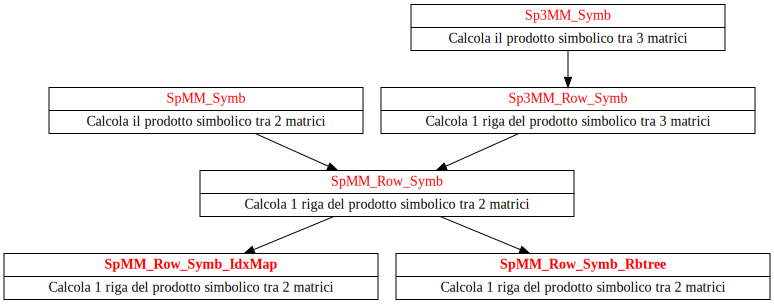
\includegraphics[width=\linewidth,keepaspectratio]{symbProductFunctionDiagram.dot.svg.pdf} \decoRule
  \label{fig:symbProductFunctionDiagram}
\end{figure}
\label{SpMM_Row_Symb_}
È possibile notare come la funzione per determinare una riga del prodotto simbolico tra 2 matrici,
\verb|SpMM_Row_Symb_|, sia alla base di tutte le altre.\\ %TODO TRIVIAL?

\subsubsection{Generazione versioni differenti di funzione}
%per Massimizzazione del riuso del codice e dell'efficienza} %TODO better title end?
%Il prodotto numerico necessità dei diversi livelli di informazione sulla matrice risultante 
%introdotti precedentemente (\refbf{chSpMMSymb:outputDetailLevel}
%per poter essere implementato con determinati approcci, come verrà descritto nel dettaglio in \refbf{chSpMMNum:funcsMultiImplePurpose}.\\
%
Al fine di massimizzare l'efficienza delle implementazioni e il riuso del codice scritto 
per generare i vari livelli di output del prodotto simbolico (descritti in \refbf{chSpMMSymb:outputDetailLevel})
ho associato alle funzione descritte in figura \refbf{fig:symbProductFunctionDiagram} 
versioni differenti, associate a delle funzionalità aggiuntive.\\
\label{chSpMMSymb:outputDetailLevel_coreFuncsVersions}
Di seguito le versioni alternative delle funzioni per eseguire la fase simbolica di SpMM e Sp3MM con specifici livelli di output,
\begin{itemize}
	\item	\verb|OutIdxs_|:
	verranno ritornati, oltre che il \nnnz di ogni (partizione di) riga della matrice risultante,
	anche i relativi indici degli elementi non zero. %della matrice risultante
	\\ \\
	Queste versioni sono necessarie per calcolare il triplo prodotto simbolico,
	come verrà descritto in \refbf{chSpMMSymb:Sp3MMSymb}.\\
	Inoltre, sono utili anche ad ottenere direttamente gli indici 
	degli elementi \nnz della matrice risultante (di cui i valori effettivi corrispondenti verranno computati nella fase numerica).\\

	\item	\verb|ColParts_|
	verranno ritornati, oltre che il \nnnz di ogni riga della matrice risultante,
	anche la loro distribuzione per ogni partizione di colonne di ogni riga. %della matrice risultante,
	\\ \\ 
	Queste versioni sono necessarie per eseguire SpMM con un partizionamento bidimensionale dei dati
	come verrà descritto in \refbf{chSpMMNum:parti2D}.\\

\end{itemize}

Le implementazioni aggiuntive appena descritte sono ottenute automaticamente 
a tempo di preprocessamento dalle funzioni base elencate in figura \refbf{fig:symbProductFunctionDiagram}
mediante l'uso delle direttive del pre-processore C \verb|#if| e molteplici \verb|#include| dei file sorgenti \citebf{cpp11.2}.
I dettagli a riguardo di questa tecnica saranno analizzati in \refbf{chSpMMAux:multiImplMany}.\\
% TODO TODO branch predictors (su path perfettamente predicibile \forall thread) + OutOfOrder exe possono rendere overhead di implementazione 
% TODO TODO con flag per livello dettaglio output e serie di if espliciti sostanzialmente con stesse performance di versione con multiple implementazioni
% TODO TODO tuttavia l'assenza di quei branch nei sorgenti può portare a maggiori ottimizzazioni in compilazione. uncomment ready ;)
%%\subsubsection{Confronto con un semplice approccio funzionale}
\label{chSpMMSymb:funcsMultiImpleVSmanualMultiFunc}
%%Nel caso di implementare la funzione \verb|SpMM_Row_Symb_|, alla base del Prodotto Simbolico accurato \refbf{chSpMMSymb:accurateBaseBlock},
%%è possibile paragonare questa metodologia implementativa ad un approccio funzionale in cui le varie versioni 
%%necessarie sono implementate in una funzione singola, componendo sotto funzioni ausiliarie e blocchi di codice su necessità con l'ausilio di \vvv{if}.
%%La speculatività dei processori moderni mediante branch predictor e esecuzione OutOfOrder può portare questa soluzione alternativa ad avere
%%potenzialmente a performance simili rispetto a quelle ottenibili da un codice in cui le istruzioni di branch sono assenti.
%%Tuttavia, la mia soluzione basata su implementazioni multiple, produrra un codice con meno branch, e di conseguenza più ottimizzabile in compilazione.\\
Quest approccio implementativo può portare a diversi benefici, come:
\begin{itemize}
	\item In casi in cui si debba traversare una struttura di indici di supporto
		  è possibile,  con una singola passata, 
		  sia copiare gli indici che tenerne traccia della loro distribuzione in partizioni separate 

	\item Considerando un'altra soluzione, basata su una singola funzione che realizza le varie  %TODO remove?
		  funzionalità richieste per il tipo di output necessario mediante delle condizioni su dei flag come approccio implementativo alternativo.\\
		  Il codice prodotto dal mio approccio implementativo, in seguito alla fase di pre processamento, gode di:
	\begin{itemize}
		\item assenza di tutte le extra istruzioni di branch richieste dall'approccio alternativo. 
			  In questo modo è potenzialmente più ottimizzabile in fase di compilazione.
			  %Tuttavia, escludendo queste ottimizzazione di compilazione, a livello teorico 
			  %la speculatività dei processori moderni mediante branch predictor e OutOfOrder execution, può portare a performance simili
		\item l'uso di meno argomenti per chiamare alcune versioni generate 
			  %% TODO TODO TODO TODO ?? ,che per molte architteture si traduce in meno passaggio dati tra memoria e registri.\\
		\item l'esclusione completa delle istruzioni non necessarie ad ogni versione generata.
	\end{itemize}
\end{itemize}
\label{chSpMMSymb:SpMM_Row_Symb_targetBaseFunc}
Di seguito la realizzazione specifica delle varie versioni della calcolo di una riga del prodotto simbolico,
ovvero la funzione \verb|SpMM_Row_Symb_| vista precedentemnte nello schema \refbf{SpMM_Row_Symb_},
in base alla struttura di supporto usata per mantenere gli indici degli elementi non zero. 
%la determinazione degli indici degli elementi \nnz di una riga di C (funzione alla base della realizzazione parallela del Prodotto Simbolico, \refbf{chSpMMSymb:accurateBaseBlock})
\subsection{Uso di RedBlack tree} \label{chSpMMSymb:usoRBTree}
Usare in parallelo una implementazione di PriorityQueue è un approccio comune
per gestire il mantenimento degli indici \nnz per il Prodotto Simbolico, come fatto da \citebf{SpMM_KNL_Multicore_symbsSols}.\\
%Dato il pattern di accesso write-mostly %TODO better CHECKKKK ANd explain
%della fase simbolica dell'operazione di SpMM ho deciso di utilizzare dei RedBlack tree piuttosto che degl'alberi AVL.\\
Tra le varie possibilità disponibili, ho scelto di usare una implementazione di RedBlack tree,
che ho ricavato personalmente dalla implementazione disponibile nel kernel Linux 5.10.85 (LTS),
mediante un processo di porting in user-space.
Il porting in userspace che ho realizzato dei RedBlack tree di linux è disponibile 
nella mia pagina: \url{https://github.com/andreadiiorio/redblackTree_linux_userspace} per altri usi.\\
Dettagli specifici dell'implementazione dei RedBlack tree e del loro processo di adattamento saranno trattati successivamente in \refbf{chSpMMAux:linuxRBTree}.\\
%Implementazioni con RBtree 
\voidLine
%operativamente uso:
Per realizzare la funzione target \verb|SpMM_Row_Symb_| con i RedBlack tree in parallelo ho assegnato al thread in esecuzione: 
1 riga di A (corrispondente alla riga target di C) ed 
un RedBlack tree allocato con un numero di nodi sufficiente per la riga più lunga di C,
%La riga più lunga della matrice risultante, necessaria per l'implementazione parallela target è 
determinata con una riduzione sul risultato di un UpperBound  del prodotto simbolico (visto in \refbf{chSpMMSymb:UpperBound}),
con livello informativo dell'output 1 (rispetto alla numerazione introdotta in \refbf{chSpMMSymb:outputDetailLevel}).\\
Durante la scansione degli indici $i$ degli elementi \nnz di B, corrispondenti agli elementi \nnz di una riga di A, 
viene effettuato un inserimento di un nuovo nodo con chiave $i$ nel RedBlack tree, se tale chiave non è stata già inserita.
Ogni inserimento avvenuto incrementa il contatore degli elementi \nnz della riga target di C.\\
Per implementare le versioni della funzione target che ritornino anche 
gli indici \nnz effettivi della riga di C (\verb|OutIdxs_|) e la loro distribuzione in partizioni di colonne (\verb|ColParts_|) è sufficiente effettuare 
una singola scansione ordinata delle chiavi $k$ inserite nel RedBlack tree prodotto, andando rispettivamente 
a salvare $k$ e/o incrementare un contatore relativo alla partizione di colonne contente $k$.\\
%altro remark di vantaggio = singola passata di rbtree dato l'approccio multi implementazione con cpp
Come già detto la scansione è singola e senza branch relativi a quale versione di \\ \verb|SpMM_Row_Symb_| si sta eseguendo grazie all'approccio
di generazione automatica di diverse implementazioni mediante pre processore.\\
\label{OUT_IDXS_RBTREE_NODES}
Nel caso di eseguire una versione della funzione in oggetto
 che ritorni gli indici degli elementi \nnz della riga risultante, %con \verb|OutIdxs_| nel suffisso del nome,
 il salvataggio della chiave $k$ del RedBlack tree generato,
può avvenire in un array di supporto, allocato precedentemente alla funzione, o 
in alternativa può essere ordinato l'array di nodi RedBlack tree dato in input, \emph{inplace}, 
contenente gli indici degli elementi \nnz della riga target di C come chiavi,
come è possibile vedere nella funzione successiva.\\
%example: building block func signature.
\begin{lstlisting}
static inline idx_t CAT4(SpMM_Row_Symb_Rbtree,OUT_IDXS,COL_PARTS,OFF_F)
  (
   idx_t* aRowJA, idx_t aRowLen, spmat* b,rbRoot* root, rbNode* nodes
   #if _OUT_IDXS  == TRUE && !defined OUT_IDXS_RBTREE_NODES 
   ,idx_t* outIdxs
   #endif
   #if _COL_PARTS == TRUE
   ,ushort gridCols,idx_t* rowColPartsLens
   #endif
  )
\end{lstlisting}
Nel frammento di codice precedente è possibile vedere come la segnatura della funzione in analisi vari in base alla versione da realizzare.
In particolare, il salvataggio degli indici \nnz degli elementi della riga target di C (versione \verb|OutIdxs_|), avviene sull'array di supporto 
\verb|outIdxs| a meno che sia definita la macro di configurazione \verb|OUT_IDXS_RBTREE_NODES|, che comporterà il riordinamento inplace del vettore di 
nodi RedBlack tree \vvv{nodes}, contente gli indici target come chiavi.\\


\subsection{Uso di bitmap di indici o array di flag} \label{chSpMMSymb:structFlagSet}
Usare una struttura contente un insieme di flag indicanti
la presenza di indici è un approccio alternativo ai RedBlack
per realizzare la funzione target \verb|SpMM_Row_Symb_| descritta in \refbf{chSpMMSymb:SpMM_Row_Symb_targetBaseFunc}, 
potenzialmente con dei benefici prestazionali per alcune versioni.\\
Analogamente al caso dei RedBlack tree, viene assegnato al thread in esecuzione 
1 riga di A, corrispondente alla riga target di C e 
un set di flag, inizializzati a false, di dimensione pari al numero di colonne $N$ di C,
sufficiente a contenere entries per ogni possibile indice della riga target di C.\\
Durante la scansione degli indici di colonna $i$ degli elementi \nnz di B corrispondenti a una riga di A, 
viene posto a true l'$i$-esimo flag e, se non era precedentemente posto false, viene anche incrementato il 
contatore degli elementi \nnz della riga target di C.\\
%macro config per scegliere struttura per set di flag
La struttura contenete il set di flag relativi agli elementi \nnz di una riga di C 
è definita nel tipo \verb|nnz_idxs_flags_t| ed è 
configurabile a tempo di compilazione mediante la macro di configurazione \verb|SPVECT_IDX_BITWISE|.
\subsubsection{bitmap di indici}		\label{chSpMMSymb:bitmapsUse}
Se la macro di configurazione \verb|SPVECT_IDX_BITWISE| è settata a \vvv{TRUE}, l'approccio usato sarà quello 
di salvare ogni indice di elementi \nnz all'interno di un insieme di bitmaps.\\
Ogni indice da inserire sarà mappato in un bit specifico, da asserire ad 1, all'interno di una delle variabili del set di bitmaps.
%bitmap sizeing
Nel caso peggiore il set di indici da inserire varia in $(0,N)$, dove $N$ può essere molto grande.\\ 
Usando varibili di dimensione $b$ bits è necessario allocarne al più $\left\lceil \frac{N}{b}  \right\rceil$
per essere in grado di poter mappare l'intero set di indici.\\
Questo approccio è usato sia nel Prodotto Simbolico che Numerico e dettagli ulteriori sull'inserimento e controllo 
di indici nelle bitmaps saranno analizzati in \refbf{chSpMMAux:bitmapInsert}.\\
Nel caso di dover realizzare efficientemente la versione \verb|OutIdxs_| della funzione target(descritta in \refbf{chSpMMSymb:outputDetailLevel_coreFuncsVersions}), 
è necessario utilizzare una struttura di supporto per salvare tutti gli indici degli elementi \nnz
 che sono stati effettivamente inseriti in una bitmap.
Per per ottemperare a questa necessità ho implementato 2 soluzioni, selezionabili a tempo di compilazione con
la macro di configurazione \verb|IDX_RMUL_SYMB_RBTREE|.\\
\begin{itemize}
	\item se \verb|IDX_RMUL_SYMB_RBTREE| è configurata a \vvv{TRUE}, tutti gli indici da salvare saranno 
		  inseriti in un RedBlack tree, per poi essere successivamente salvati ordinatamente in un array pre allocato
		  da ritornare.
	\item se \verb|IDX_RMUL_SYMB_RBTREE| è configurata a \vvv{FALSE}, tutti gli indici da salvare saranno inseriti
		  (in ordine casuale dipendente dai non zeri delle matrici considerate) direttamente nell'array da ritornare
		  per poi essere ordinati.
\end{itemize}
Entrambi questi approcci hanno un costo computazionale pari a $O(n log n)$ dove n è il numero di indici inseriti.\\

\subsubsection{Array di flag}
Alternativamente, se la macro di configurazione \verb|SPVECT_IDX_BITWISE| è settata a FALSE, 
ho realizzato un approccio più semplice, basato su un array di $N$ $char$, 
dove l'indice di colonna $i$ da inserire corrisponde ad un valore non zero nel $i$-esimo elemento dell'array.
La gestione della versione \verb|OutIdxs_| della funzione target è analoga al caso precedente.\\  %trivial?

\subsection{Sp3MM: Calcolo simbolico diretto del triplo prodotto} \label{chSpMMSymb:Sp3MMSymb}
Dato che il problema orinario da risolvere è il triplo prodotto tra matrici sparse per applicazioni come 
amg4psblas \citebf{AMG4PSBLAS}, ho deciso di cercare di supportare anche la moltiplicazione diretta 
tra 3 matrici sparse, con un'estensione della formulazione row-by-row.\\
Seguendo la notazione introdotta inizialmente in \refbf{notazione}, l'approccio seguito è derivato da quello seguito da \citebf{Sp3MM4AMG}.\\
Una volta computata la riga $\left(R\cdot AC_i\right)_{r*}$ con la versione \verb|OutIdxs_| di \verb|SpMM_Row_Symb_|, 
questa viene riutilizzata direttamente nel prodotto con la matrice $P$, analogamente al caso di SpMM,
per ottenere la dimensione della riga relativa della matrice risultante ${AC_{i+1}}_{r*}$ ed eventualmente anche altre informazioni.\\ 
Le versioni \verb|OutIdxs_| sono necessarie per ottenere \\gli indici di colonne della riga $\left(R\cdot AC_i\right)_{r*}$,
indispensabili per reiterare la formulazione \rowbyrow sulla matrice $P$.\\
L'operazione appena descritta è eseguita in parallelo per ogni riga di $AC_{i+1}$.\\
%Determinare la quantità di elementi \nnz è possibile incontrare durante i primi prodotti tra le righe di $R$ e $AC_i$ è necessario 

\subsection{Pro e contro UpperBound vs Prodotto Simbolico Accurato} \label{chSpMMSymb:UB_VS_SYMBACC}
L'analisi delle differenze prestazionali delle implementazioni di SpMM con fase Simbolica Accurata o UpperBound
sarà analizzata in seguito nel capitolo \refbf{ChPerf}.\\
Di seguto qualche considerazione di carattere generale che è possibile trarre dall'analisi di questi approcci differenti
al problema di Sp[3]MM.\\
\begin{enumerate}
	\item L'UpperBound gode sicuramente di un costo computazione nettamente inferiore 
	      rispetto a qualsiasi implementazione di Prodotto Simbolico accurato.\\
	\item Tuttavia, questo vantaggio iniziale per soluzioni basate su UpperBound, 
		  è associato alla necessità di dover salvare tutti i risultati intermedi in una struttura temporanea,
		  di cui è necessario effettuare una copia nella matrice risultante.
	\begin{enumerate}
		\item Viceversa il Pro dotto Simbolico accurato permette di poter salvare tutti i risultati intermedi,
			  ottenuti durante la fase Numerica, direttamente nella matrice risultante.
	\end{enumerate}
	\item Il Prodotto Simbolico  accurato di $A \cdot B$, 
		  basato su una formul azione derivata da gustavson \citebf{gustavson}, ad esempio row-by-ro,
		  soffre di un ulteriore svantaggio dovuto a dover accedere le righe $B$ in un ordine casuale, derivato 
		  dagli indici degli elementi \nnz della riga corrispondente di A.\\
		  Questo causa potenzialmente un cattivo uso della memoria, come analizzato da 
		  \citebf{Sp3MM4AMG} ed indirettamente da \citebf{ESC}.
		\begin{enumerate}
			\label{chSpMMSymb:UB_VS_SYMBACC_rowbyrowContiguousCopyBack}
			\item Viceversa, il costo addizionale legato allo svantaggio dell'uso di UpperBound menzionato al punto 2, 
				  comporta la copia di risultati intermedi 
				  nella matrice risultante in maniera contigua, come osservato da \citebf{Sp3MM4AMG}
		\end{enumerate}
	\item In generale, l'overhead di memoria causato dall'UpperBound, potrebbe essere tale da rendere impossibile 
		  sfruttare su GPU una fase simbolica basata su UpperBound. %come osservato da \citebf{TODO ritrovalo}
\end{enumerate}
